\section{Theory}
\label{sec:theory}

This section is devoted to laying out a more formal description of the
theory presented in Section~\ref{sec:intro}. While the particles and
their properties tabulated in Figure~\ref{fig:sm} summarize the important
players in the study of elementary particles, an understanding of the
mathematical ideas behind the Standard Model's construction are essential in grasping
the importance of this measurement. This paper is focused on the measurement
of \HToZg at the LHC; therefore, a rigorous development of this ideas is forgone. 
For this see Halzen and Martin~\cite{QuarksLeptons}.

% Section~\ref{subsec:qed} gives a brief
% introduction to Gauge Theory and Quantum Field Theory through the simplest
% theory contained in the Standard Model: Quantum Electrodynamics (QED).
% Afterward the Higgs Mechanism is explained in Section~\ref{subsec:higgsmec}
% and finally the production processes studied in this measurement are
% given in Section~\ref{subsec:prodproc}.


\subsection{The Role of Symmetry in Particle Physics}
\label{subsec:symmetry}

An important principle motivating the mathematical structure of modern physical 
theories is the notion of symmetry. On a macroscopic scale one can study
the interactions of objects by holding them at various
distances apart and measuring the force between them. That is how Coulomb derived
the famous inverse square law describing electric repulsion and attraction that
now bears his name. On the smallest scales this empirical data is no longer
available, so that a new paradigm is need to understand how these interactions
come about. 

A beautiful solution was brought to light by the brilliant 
mathematician and physicist Emmy Noether who showed that every symmetry in
nature leads to a conserved quantity, a value that does not change over time.
A familiar application of this connection is found in Newton's third law:
For every action there is an equal and opposite reaction. From this balancing of
forces one can derive a conserved quantity associated with the system's 
motion, namely momentum. The importance of Noether's approach using symmetries
is that it allows the physicist to turn this reasoning around. One can postulate
the existence of a symmetry of nature, in this case the invariance of the laws
of physics under translations in space, which leads to a conserved quantity (momentum)
that results in experimentally testable predictions (Newton's third law).

While quantities such as momentum are familiar at the macroscopic level, 
it turns out that similar symmetries exist at subatomic distances
known as internal symmetries. One of the first examples of these symmetries
known as isospin was put forth by Werner Heisenberg in 1932 
to explain the approximate symmetry between
the newly discovered neutron with its partner in the atomic nucleus, the proton.
This symmetry says that according to the strong interaction that holds
the nucleus together the neutron and proton are reflections of each other,
i.e. the exchange proton $\leftrightarrow$ neutron does not affect the
physics of the strong force. More importantly this symmetry predicts that the
scattering rates of the interactions
\begin{align*}
    & p + p \rightarrow \pi^+ + d \\
    & p + n \rightarrow \underbrace{\pi^0}_{\text{pion}} + \underbrace{d}_{\text{deuteron}}
\end{align*}
should be equal. The experimental verification of this prediction convinced
physicists that these internal symmetries can be used to study and predict
how particles interact at the smallest length scales.

Physicists now use similar internal symmetries known as gauge symmetries to
describe the fundamental particles and their interactions. These gauge symmetries
are mathematical constructs similar to isospin that predict force carrying 
particles that mediate interactions in a way that can be used to calculate
various measurable quantities. The current gauge-theory formulation which describes
much of the phenomena found in nature is known as the Standard Model.

\subsection{The Standard Model}
\label{subsec:StandardModel}
An picture of the Standard Model of particle physics is best obtained
by moving away from the abstract gauge-theory formulation and instead considering
the predictive outcomes of the theory. The Standard Model provides physicists with
the current answer to the question of what the world is made of and is displayed
in Figure~\ref{fig:sm}. This table is reminiscent
of the periodic table developed by chemists to explain the various atoms
found in nature. A surprising property of the Standard Model is that it consists
of only 16 different particles. There are six quarks, shown in purple, which
are the building blocks of the familiar nucleons, i.e. the proton and neutron.
Another six particles known as leptons, marked in green, include one of
the most familiar fundamental particles, the electron, 
which is responsible for the operation of most household circuits. And
finally there are the four gauge bosons highlighted in red, which are of the 
greatest relevance to the measurement presented in this paper.
The gauge bosons are responsible for mediating three 
out of the four fundamental forces in nature: the electromagnetic, strong, and 
weak interactions. As of now, theorists have been unable to incorporate the 
gravitational force, a pervasive component of the macroscopic world,
into the current gauge-theory of particle physics.

\begin{figure}[htbp]
    \centering
    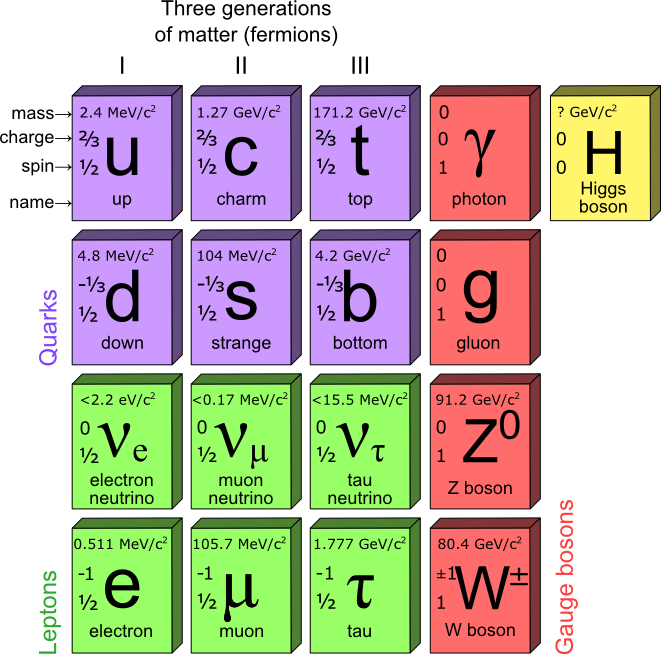
\includegraphics[scale=0.4, angle=0]{./figures/StandardModelPNG}
    \caption{A table summarizing the particles described by the
    Standard Model of particle physics. The Standard Model encompasses
    three generations of quarks and leptons as well as four force carrying
    bosons.}
    \label{fig:sm}
\end{figure}

\subsection{The Higgs Mechanism}
\label{subsec:higgsmec}
The Higgs boson is an essential component of the Standard Model and plays
an important role in the predictive power of the theory. Like much of modern
physics, the Standard Model relies heavily on the symmetries of nature. Just
as concepts such as conservation of momentum and energy can be tied to the 
fact that a system is symmetric under translations in space and time\footnote{
This result is known as Noether's Theorem and can be attributed to the 
brilliant German mathematician Emmy Noether.}, much of the mathematical 
framework of the Standard Model is based on internal symmetries 
known as gauge symmetries. In fact there are three gauge symmetries found
in the Standard Model\footnote{ In group theoretic language the symmetries of
the Standard Model can be written as $SU(3) \times SU(2) \times U(1)$.} 
each of which predicts a force carrying particle that mediates one of the 
aforementioned interactions of nature. The photon mediates the 
electromagnetic interaction. The massless gluon is responsible for the strong 
interaction, which binds quarks together to form protons and neutrons.
And finally, the weak interaction, which causes radioactive decays, 
is mediated by the massive \WBosons and \ZBoson bosons. The problem with all 
of this symmetry is that it predicts that the weak nuclear force is a long
range force, something which is not observed in nature. The reason for this
discrepancy can be traced back to the fact that the \WBoson and \ZBoson bosons are
not massless particles, but have a mass of roughly 80 and 90 GeV respectively. 
In addition, these internal gauge symmetries also predict that other 
fundamental particles, such as the electron, are massless. In order to solve
this apparent predicament one needs to introduce a mechanism that keeps the
equations that govern the Standard Model's behavior symmetric, but allows for
some asymmetric lowest energy states, i.e. 'ground states'. 
This is accomplished with a theoretical mechanism known as spontaneous
symmetry breaking or in this special case the Higgs mechanism.

\subsection{Production Process}
\label{subsec:prodproc}

\begin{figure}[!htbp]
  \begin{center}
  {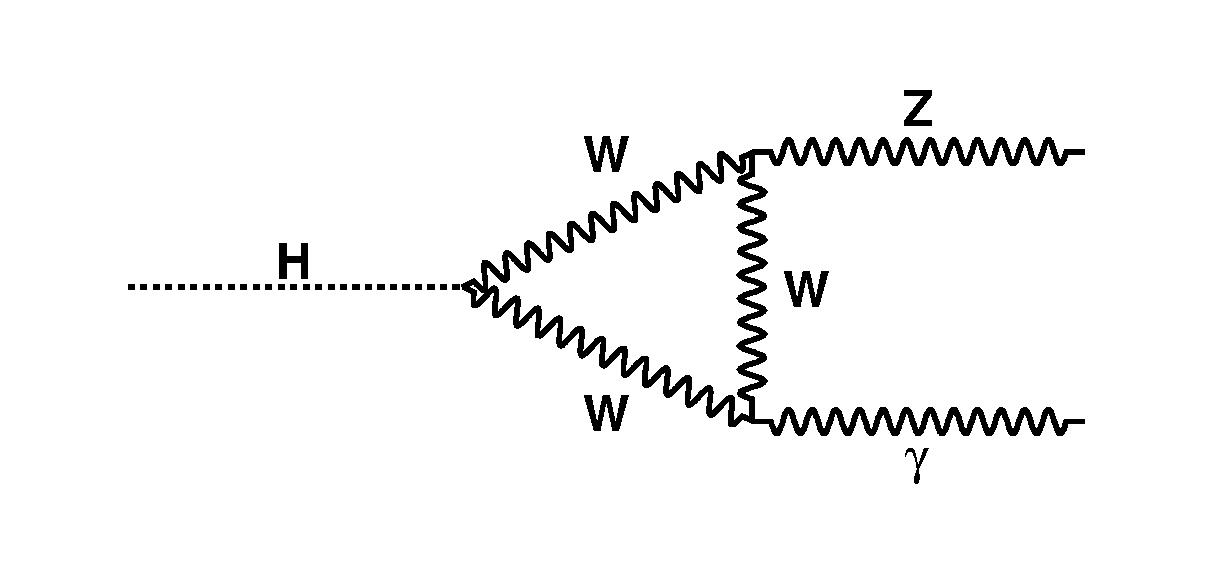
\includegraphics[width=2in]{figures/loop1}}
  {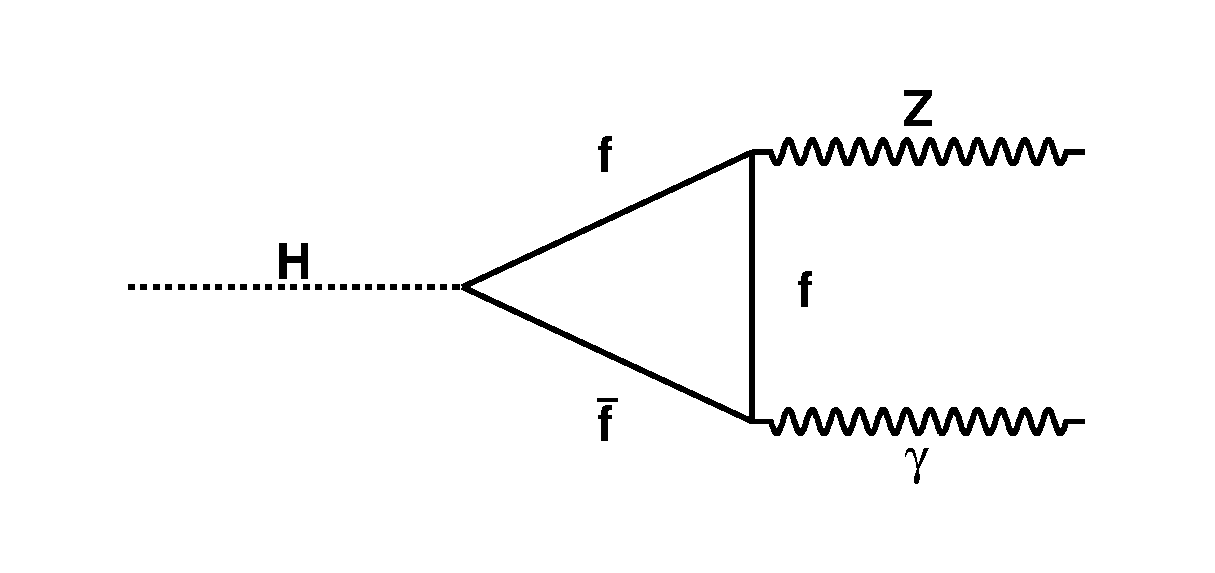
\includegraphics[width=2in]{figures/loop2}}
  {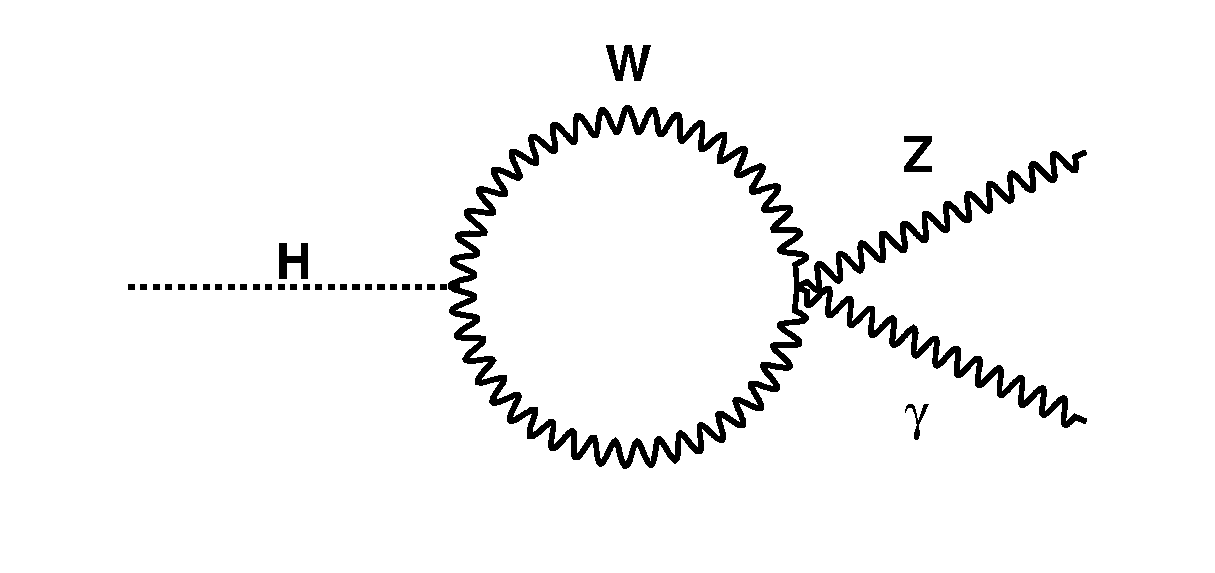
\includegraphics[width=2in]{figures/loop3}}
  \caption{Leading Feynman diagrams for the $H\rightarrow Z\gamma$
    decay in the Standard Model. Note that in the case of the fermion
    loop, top quarks dominate.} 
  \label{fig:feynman}
  \end{center}
\end{figure}

% There are many ways to analyze the dynamics of a particle classically; however,
% the one most suited for studying the symmetries of a system is Lagrangian Mechanics.
% The study of such a systems begins by defining a Lagrangian function as
% \begin{equation}
%     L(q, \dot q) = T - U 
% \end{equation}
% where $T$ and $U$ are the particle's kinetic and potential energy respectively, 
% so that the Lagrangian is a function of the particle's coordinates and velocities. 
% The mathematics behind the Standard Model is formulated in terms of the Langrian
% approach to mechanics; however, a minor detail arises because the Standard Model
% describes fields not particles.
% 
% The Standard Model is a Quantum Field Theory meaning that it is not interested in
% describing particles, which are localized entities, but in describing the
% dynamics of fields, which occupy some extended region of space. For example the
% electromagnetic field $\mathbf{E}$ is a vector vield that is described 
% by three component functions that can change throughout space and time: 
% $\mathbf{E}(\phi_i) = (\,\phi_x(x,y,z,t), \phi_y(x,y,z,t), \phi_z(x,y,z,t)\,)$. 
% As such the Lagrangians contained in the Standard Model are functions of these
% fields and their derivative.
% 
% As an introduction to how these mathematical formalism works let's consider the
% Lagrangian descibing QED:
% \begin{equation}
% \mathcal{L} = \frac{-1}{16\pi}\left(\partial^{\mu} A^{\nu} - \partial^{\nu}A^{\mu}\right) = 
% \frac{-1}{16\pi} F^{\mu\nu}F_{\mu\nu}.
% \end{equation}
% were $A^{\mu} = (\phi, \mathbf{A})$ is the electomagnetic potential.
